\documentclass[english,10pt,handout]{beamer}
%\documentclass[english,10pt]{beamer}

\usepackage[clock]{ifsym}
%\usepackage{clock}






 
%\usepackage{mathptmx}
%\renewcommand{\sfdefault}{lmss}
\usepackage[T1]{fontenc}
%\usepackage[latin9]{inputenc}
\usepackage[utf8]{inputenc}

\synctex=-1

\usefonttheme{professionalfonts}

%\setbeamertemplate{navigation symbols}{}
%\setbeamertemplate{caption}[numbered]


\useinnertheme{rectangles}
%http://tex.stackexchange.com/questions/11168/change-bullet-style-formatting-in-beamer

 \AtBeginDocument{
  \addtolength\abovedisplayskip{-0.4\baselineskip}%
  \addtolength\belowdisplayskip{-0.4\baselineskip}%
}%change the space between text lines and the math formula


\usepackage{pifont}
%Postscript ZipfDingbats font
%the command \ding{number}, will print the specified symbol

\usepackage{fontawesome}
%icon package
\DeclareFontFamily{U}{FontAwesomeOne}{}
\DeclareFontShape{U}{FontAwesomeOne}{m}{n}{<-> FontAwesome--fontawesomeone}{}
\DeclareRobustCommand\FAone{\fontencoding{U}\fontfamily{FontAwesomeOne}\fontseries{m}\fontshape{n}\selectfont}
\DeclareFontFamily{U}{FontAwesomeTwo}{}
\DeclareFontShape{U}{FontAwesomeTwo}{m}{n}{<-> FontAwesome--fontawesometwo}{}
\DeclareRobustCommand\FAtwo{\fontencoding{U}\fontfamily{FontAwesomeTwo}\fontseries{m}\fontshape{n}\selectfont}
\DeclareFontFamily{U}{FontAwesomeThree}{}
\DeclareFontShape{U}{FontAwesomeThree}{m}{n}{<-> FontAwesome--fontawesomethree}{}
\DeclareRobustCommand\FAthree{\fontencoding{U}\fontfamily{FontAwesomeThree}\fontseries{m}\fontshape{n}\selectfont}

%ftp://ftp.dante.de/tex-archive/fonts/fontawesome/doc/fontawesome.pdf
%http://tug.ctan.org/info/symbols/comprehensive/symbols-a4.pdf


\usepackage{amsmath,amssymb,amsfonts,bm,mathrsfs,mathtools}

\usepackage{tikzsymbols}
%\usepackage[tikz]{bclogo}



\usepackage{perpage}
\MakePerPage{footnote} %reset for each page
%\renewcommand{\thefootnote}{\fnsymbol{footnote}} %use symbol, limit less than 9 symbols



%%%% HIGHTLIGHT  and annotation &=%%%%%%%%
\usepackage{color,xcolor}
 \usepackage{todonotes}

\usepackage[normalem]{ulem}

\usepackage[many]{tcolorbox}

\tcbset{fonttitle=\scriptsize}
\tcbset{highlight math style={enhanced,
  colframe=red!40!black,colback=yellow!20!white,arc=2pt,boxrule=.2pt,
  }}
  \newtcbox{\otherbox}[1][]{nobeforeafter,math upper,tcbox raise base,
enhanced,frame hidden,boxrule=0pt,interior style={top color=green!10!white,
bottom color=green!10!white,middle color=green!50!yellow},
fuzzy halo=1pt with green,#1}
%%\tcbhighmath{math here}
%% \otherbox{math here}



%%%%% HIGHLIGHT %%%%%%
\newcommand{\hb}[1]{{\color{blue}{#1}}}
%\noindent\rule{\textwidth}{.5pt}

%:
\usepackage{soul}

\newcommand\hcancel[2][black]{\setbox0=\hbox{$#2$}%
\rlap{\raisebox{.45\ht0}{\textcolor{#1}{\rule{\wd0}{1pt}}}}#2}
%cross to delete

\newcommand{\mcb}[2]{\colorbox{#1}{$\displaystyle #2$}}
%highlight math

\newcommand{\hlfancy}[2]{\sethlcolor{#1}\hl{#2}}
%specified color , for\hl

\newcommand\myhl{\bgroup\markoverwith
  {\textcolor{yellow}{\rule[-.5ex]{2pt}{2.5ex}}}\ULon}



\mode<presentation>{ \usetheme{boxes} }

%write Matlab code
\usepackage{listings}
 \definecolor{dkgreen}{rgb}{0,0.6,0}
\definecolor{gray}{rgb}{0.5,0.5,0.5}
\definecolor{mauve}{rgb}{0.58,0,0.82}
\lstset{frame=tb,
  language=Matlab,
  aboveskip=3mm,
  belowskip=3mm,
  showstringspaces=false,
  columns=flexible,
  basicstyle={\small\ttfamily},
  numbers=none,
  numberstyle=\tiny\color{gray},
  keywordstyle=\color{blue},
  commentstyle=\color{dkgreen},
  stringstyle=\color{mauve},
  breaklines=true,
  breakatwhitespace=true
  tabsize=3
}

\usepackage[lastexercise]{exercise}

\newtheorem{ex}{Exercise}
\newtheorem{property}{Property}
\newtheorem{ag}{Algorithm}
\newtheorem{remark}{Remark}
\newtheorem{den}{definition}
\newtheorem{assumption}{Assumption}


\usepackage[nosolutionfiles]{answers}
\Newassociation{sol}{Solution}{ans}



\usepackage{empheq}
\usepackage{comment}
%\usepackage{lscape}
\usepackage{multirow}
\usepackage{url,hyperref}

\hypersetup{
 %   bookmarks=true,         % show bookmarks bar?
    unicode=false,          % non-Latin characters in Acrobat's bookmarks
    pdftoolbar=true,        % show Acrobat's toolbar?
    pdfmenubar=true,        % show Acrobat's menu?
    pdffitwindow=false,     % window fit to page when opened
    pdfstartview={FitH},    % fits the width of the page to the window
    pdftitle={My title},    % title
    pdfauthor={Author},     % author
    pdfsubject={Subject},   % subject of the document
    pdfcreator={Creator},   % creator of the document
    pdfproducer={Producer}, % producer of the document
    pdfkeywords={keyword1} {key2} {key3}, % list of keywords
    pdfnewwindow=true,      % links in new window
    colorlinks=true,       % false: boxed links; true: colored links
    linkcolor=red,          % color of internal links (change box color with linkbordercolor)
    citecolor=green,        % color of links to bibliography
    filecolor=magenta,      % color of file links
    urlcolor=cyan           % color of external links
}


\usepackage{subfigure,epsfig,graphicx,graphics}

\DeclareGraphicsRule{.tif}{png}{.png}{`convert #1 `dirname #1`/`basename #1 .tif`.png}
   \DeclareGraphicsExtensions{.pdf}




\newcommand{\hw}{ {\underline{\tt Homework }} }
\newcommand{\hws}{ {\underline{\tt Homework$\star$}} }
\newcommand{\optional}{ {\it optional} }

\newcommand{\MATLAB}{ \texttt{MATLAB}}
\newcommand{\python}{ \texttt{python}}
\newcommand{\Rlang}{ \texttt{R}}
\newcommand{\SAS}{ \texttt{SAS}}
\newcommand{\MC}{Markov Chain}


\newcommand{\tm}{transition matrix}
\newcommand{\rv}{random variable}
\newcommand{\spl} {supervised learning }
 

\newcommand{\dis}{\underline{\tt discussion}: }
\newcommand{\pri}{\underline{\tt principle}: }




\newcommand{\bq}{\scalebox{6}{\textbf{?} }}
\newcommand{\sq}{\scalebox{2}{\textbf{?} }}
\newcommand{\ck} {  {\scalebox{0.8} {\Interval}   } }

\newcommand{\eps}{\varepsilon}
\newcommand{\To}{\longrightarrow}

% 
\newcommand{\Dcal}{\mathtt{D}}
\newcommand{\Hcal}{\mathcal{H}}
\newcommand{\Ecal}{\mathcal{E}}
\newcommand{\Xcal}{\mathcal{X}}
\newcommand{\Ycal}{\mathcal{Y}}
\newcommand{\Zcal}{\mathcal{Z}}

%%Calculus 

\renewcommand{\d}{\ensuremath{\mathrm{d}}}
\newcommand{\dt}{ \ensuremath{\mathrm{d} t } }
\newcommand{\dx}{ \ensuremath{\mathrm{d} x} }
\newcommand{\dy}{ \ensuremath{\mathrm{d} y } }

%indicator function
\newcommand{\indf}{ \ensuremath{\mathbf{1} } }



%probability
\newcommand{\p}{ \mathbb{P}}
\newcommand{\prob}{{\Pr}}
\newcommand{\PP}{\mbox{PP}}%Poisson process
%condition prob
\newcommand{\cPr}[2]{{\Pr\left(#1\mid #2\right)}}

\newcommand{\FF}{{\mathbb{F}}}

\newcommand{\e}{ \operatorname{\mathbb E}}
\newcommand{\Var}{\operatorname{\mathbb{V} }}
\newcommand{\var}{\operatorname{\text{Var} }}
\newcommand{\MSE}{\operatorname{\text{MSE} }}

\newcommand{\Std}{\operatorname{std}}
\newcommand{\Cov}{\operatorname{cov}}

%Matrix  %mathbf
\newcommand{\Pb}{{\mathbf{P}}}
\newcommand{\Qb}{{\mathbf{Q}}}
\newcommand{\Mb}{{\mathbf{M}}}
\newcommand{\cb}{\mathbf{c}}
\newcommand{\bb}{{\mathbf{b}}}

\newcommand{\Tb}{\mathbf{T}}

\newcommand{\Wb}{\mathbf{W}}
\newcommand{\wb}{\mathbf{w}}
\newcommand{\Xb}{\mathbf{X}}

\newcommand{\xb}{\mathbf{x}}

\newcommand{\Wtn}{\mathbb{W}}
\newcommand{\btn}{\mathbf{b}}



\newcommand{\eye}{{\mathbf{I}}}
%identity matrix
\newcommand{\onem}{{\mathbb{1}}}
\newcommand{\idor}{\mathbf{1}}
\newcommand{\ii}{\mathbf{i}}
%imaginary symbol

\usepackage{tikz}

%State number
\newcommand{\snum}[1]{ \raisebox{.5pt}{\textcircled{\raisebox{-.9pt} {#1}}}}

 \usetikzlibrary{arrows}
\usetikzlibrary{shapes}

%\newcommand{\snum}[1]{%
 % \tikz[baseline=(char.base)]\node[anchor=south west, draw,rectangle, rounded corners, inner sep=1.4pt, minimum size=5mm,
   % text height=1.3mm](char){\ensuremath{#1}} ;}

\newcommand*\circled[1]{\tikz[baseline=(char.base)]{
            \node[shape=circle,draw,inner sep=.4pt] (char) {#1};}}


%real number
\newcommand{\Real}{{\mathbb{R}}}
%integer
\newcommand{\ZZ}{\mathbb{Z}}
%positive integer
\newcommand{\NN}{\mathbb{N}}



\newcommand{\inpd}[2]{\left\langle #1, #2 \right\rangle}
\newcommand{\abs}[1]{\left\vert#1\right\vert}
\newcommand{\norm}[1]{\left\|#1\right\|}
\newcommand{\wt}[1]{{\widetilde{#1}}}
\newcommand{\set}[1]{\left\{#1\right\}}
\newcommand{\partiald}[2]{  \frac{\partial #1 }{\partial #2}}



\newcommand{\ie}{{\it{i.e.}}}



\newcommand{\transpose}{\textsf{T}} % or, \intercal
\newcommand{\diag}{\textsf{diag}}
\newcommand{\tr}{{\textsf{T}}}
\newcommand{\rt}{{\textbf{r}}}

\DeclareMathOperator{\trace}{Trace}


\newcommand{\argmin}{ \operatornamewithlimits{argmin} }
\newcommand{\argmax}{ \operatornamewithlimits{argmax} }




\def\biz{\begin{itemize} }
\def\bizp{\begin{itemize}[<+->] }
\def\eiz{\end{itemize}}


\def\bfm{\begin{frame}}
\def\efm{\end{frame}}

\def\bena{\begin{enumerate}[<+-| alert@+>]}
\def\ben{\begin{enumerate}}
\def\een{\end{enumerate}}


\def\bbk{\begin{block} }
\def\ebk{\end{block}}






\makeatletter
%%%%%%%%%%%%%%%%%%%%%%%%%%%%%% Textclass specific LaTeX commands.
 % this default might be overridden by plain title style

%%%%%%%%%%%%%%%%%%%%%%%%%%%%%% User specified LaTeX commands.
%\usetheme{Warsaw}
\usetheme{Boadilla}
% or ...



%\setbeamertemplate{footline}[text line]{} % makes the footer EMPTY
%\setbeamertemplate{footline}[page number]{} % makes the footer EMPTY

%\usecolortheme{orchid} %not use is better 

\setbeamertemplate{footline}[text line]{%
  \parbox{\linewidth}{\vspace*{-2pt}Xiang Zhou\hfill CityU\hfill \insertpagenumber}}
%\setbeamertemplate{navigation symbols}{}

%\setbeamercovered{transparent}
% or whatever (possibly just delete it)


%\usepackage{babel}
\makeatother



 %
%\addtobeamertemplate{frametitle}{}{%
%\begin{tikzpicture}[remember picture,overlay]
%\node[anchor=south east,yshift=2pt] at (current page.south east) {
\includegraphics[height=0.6cm]{CityU_Logo_Basic_Signature.eps}};
%\end{tikzpicture}}
%

\beamerdefaultoverlayspecification{<+->}
%the presentation acts as though a \pause command has been inserted between every two bullets, without the actual need to write \pause after each item.




\title{MA4546: Introduction to Stochastic Process}

\author{
\includegraphics[height=1.1cm,width=2.2cm]{CityU_Logo_Basic_Signature.eps}
\\ $\ $ \\
Xiang Zhou  \\ $\ $ \\
}
\institute[]{Department of Mathematics
}

\date[]{2016-2017, Semester A}



\begin{document}

 \maketitle 
 
\frame{
\
{\Large Chapter 4: Continuous-Time Markov Chain}

 }



\setlength{\belowdisplayskip}{3pt} \setlength{\belowdisplayshortskip}{3pt}
\setlength{\abovedisplayskip}{3pt} \setlength{\abovedisplayshortskip}{3pt}





\frame{{CTMC}

\begin{definition}[CTMC]
A stochastic process
$\{ X(t); t\in \Real_+\}$
 on the state space $S$ \footnote{We consider finite state space most of time; occasionally we consider
 the countable infinite state space like $\mathbb{N}=\{0,1,2,3,\cdots\}$} is called a CTMC if,
 for all state $i$ and $j$ in $S$ and $t,s \geq 0$,
 \[
\p(X(s+t) = j | X(s)=i, X(u), 0\leq u\leq s) =
\p(X(s+t) = j | X(s)=i).
\]

The CTMC $\{ X(t); t\geq 0\}$
is said to be time homogeneous\footnote{We only study this time-homogeneous case.}
if for $t,s\geq 0$,
\[  \p(X(s+t) = j | X(s)=i)=
\p(X(t) = j | X(0)=i). \]

\end{definition}
 \pause
The \pp\ and compound \pp\ are both 
examples of CTMC.

}


\frame{
{Chapman-Kolmogorov equations}



\bigskip
Denote the transition matrix for $X(t)$ by 
$\Pm(t)=[P_{ij}(t)]$\footnote{We need save the notation  $``p_{ij}''$ for future use.},
where the transition  probability at time $t$ is defined as
\[ P_{ij}(t):=\Pm(t)_{ij}= \p(X(t)=j|X_0=i).\]
For each $t$, $\Pm(t)$ is a stochastic matrix on $S$ for each $t\geq 0$.

\pause
\medskip 

We have the following most important result for the family $\{\Pm(t): t\geq 0\}$
\begin{theorem}[Thm4.1]
If $\{\Pm(t): t\in \Real_+\}$ is the transient matrix of a CTMC, then
it satisfies the following    {\it   semigroup property}: that is 
\[\boxed{  \Pm(s+t) = \Pm(s)\Pm(t) = \Pm(t) \Pm(s)},~~\forall s, t \in \Real_+\]
\end{theorem}
\bigskip
  $\{\Pm(t): t\geq 0\}$  is thus called  a transition  semigroup.
  
This is an   analogy to the result for DTMC.

}


\frame{\Large  Two simple Examples of CTMC}

\frame{{ A failure model of two-state CTMC}


\begin{example}[Example 4.1]
Suppose the lifetime of a high-altitude satellite
is an Exp($\mu$) random variable. Once it fails, it stays failed forever since no repair is
possible. Let $X(t)$ be 1 if the satellite is operational at time $t$ and 0 otherwise.
The transition matrix of this process $\{\Pm(t)\}$ is 
\only<2->
{
\[
\Pm(t) = 
\begin{bmatrix}
1 & 0 \\
1 - e^{-\mu t} & e^{-\mu t}
\end{bmatrix}\]
}
\end{example}
 \only<3->
 {Please verify the  semigroup property for this example.}


\bigskip 


\only<4|handout:0>{
The state space is ?. The transition  is 
a jump from ? to ?, which is triggered \bomb\   by ?? event.
The waiting time \ck for this event is a ??? random variable.
}


\only<5->{
The state space is $\{0,1\}$. The transition  is 
a jump from ``1'' to ``0'', which is triggered by the event 
of ``failure''  \bomb. The waiting time \ck 
 for this event is an $Exp(\mu)$ random variable:
$ \p(X(t)=0\vert X(0)=1) = 1- e^{- \mu t} $.
}


\medskip
\only<6->
{\centering \tt We can understand  this example (as well as any CTMC) {\it intuitively} using what we learnt 
in Chapter 2 (DTMC) and Chapter 3 (Poisson process):    }

\only<7>{
\bbk{\centering
Wait   \ck   until   \bomb\ , then jump {\it as if} a DTMC does. 
} \ebk 
}
  
 


}

\frame{{Poisson process with parameter $\lambda$}

\begin{example}
Let $\{N(t)\}$ be a $PP(\lambda)$.
How to interpret this process using  the  above picture ?
What is the transition matrix $\{\Pm(t)\}$ for $\{N(t)\}$ ? 
\end{example}
 
\biz[<+->]
\item
The state space $S=\{0,1,2,\ldots,\}$ (countable infinite).
\item 
For any value of $N(t)$, say $N(t)=k$,   the waiting (sojourn) time 
(inter-event time interval)\ck  at this state is an $Exp(\lambda)$ \rv.
\item When the time \ck is up, \bomb\ ,  $N$ jumps to the state $k+1$.
\item  Wait the next iid random clock \ck $\sim Exp(\lambda)$  to bomb again \bomb\, ,  
$N$ makes  a jump  again to $k+2$.
\item  $\ldots$,     \ck    $\to $   \bomb\ $\to $  $N$ jumps. 
\eiz 
 
}
 
\frame{{Transition matrix of \pp}
\vspace{-5pt}
\[
\begin{split} P_{ij}(t)&= \p(N(t+s) =j)\, | N(s)=i)
\\
&=
\p(N(t+s)-N(s)=j-i) (\mbox{ Poisson r.v with parameter } ~\lambda t)
\\
&=\begin{cases}
e^{-\lambda t } \frac{ (\lambda t)^{j-i}}{ (j-i)!} & \mbox{if}~~ j \geq i,\\
0 & \mbox{if} ~~j < i.
\end{cases}
\end{split}
\]


\[
\Pm(t)=[P_{ij}(t)] =\begin{bmatrix}
e^{-\lambda t} & \lambda t e^{-\lambda t} & \frac{\lambda^2 t^2}{2!} e^{-\lambda t}  &  \frac{\lambda^3 t^3}{3!} e^{-\lambda t} & \cdots \\
0 & e^{-\lambda t} & \lambda t e^{-\lambda t} & \frac{\lambda^2 t^2}{2!} e^{-\lambda t}  & \cdots \\
0 & 0 &e^{-\lambda t }& \lambda t e^{-\lambda t}  & \cdots \\
\vdots & \vdots & \vdots & \vdots & \ddots
\end{bmatrix}
\]

\pause 

\begin{ex}
\biz
\item
 Verify the  semigroup property for this example!
 \item
If we only count each jump \bomb, regardless of the time \ck, 
we get a DTMC on S.  What is the (one-step) transition matrix, written as
$[p_{ij}]$, for this DTMC  ? 
\eiz
\end{ex}



}

\frame{
{The clock \ck   (  $Exp$ r.v.s ) can have      different rates}
The inter-event (waiting) times may have different rates which depend
on which state the system is staying.

Some clocks run   fast (large $\lambda$);  some clocks run   slow (small $\lambda$).
See example next page.
\begin{center}
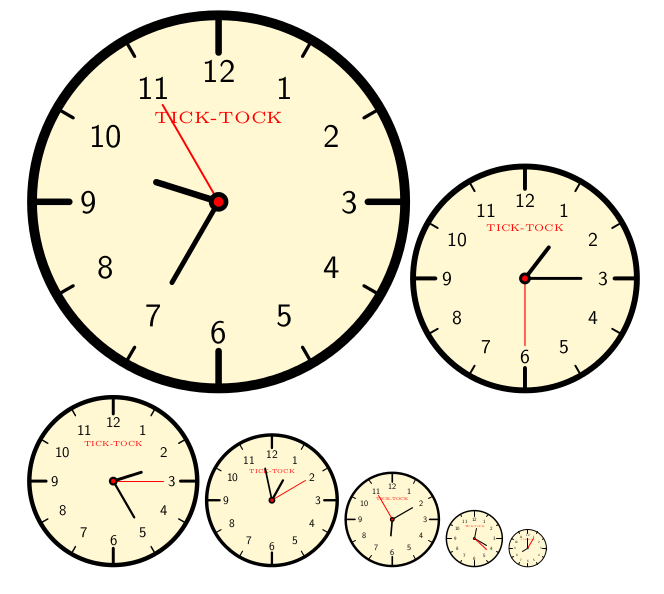
\includegraphics[width=0.6\textwidth]{clocks.png}
\end{center}

}


\frame{{   Example: Kinematics of chemical reactions}
We consider a closed system of two species of molecules, $[A]$ and $[B]$,
 where the following three chemical  reactions occur
\ben
\item $[A]\to \emptyset$  (degradation of $[A]$  ) with rate $\kappa_1=a/10$
\item $[A]\to [B]$ with rate $\kappa_2=a$
\item $[B]\to [A]$ with rare $\kappa_3=2b$
\een
where the non-negative integers  $a,b$ are the number of molecules $[A]$ and $[B]$, respectively.
\pause
This can be modelled as CTMC. 
The state space is $S= \{(a,b)\in \mathbb{Z}^2 :  a\geq 0, b\geq 0\}$.
Each reaction correspond to one   event: 
\ben[<+->]
\item for Reaction (1): $(a,b)\to (a-1, b)$;
\item for Reaction (2): $(a,b)\to (a-1, b+1)$;
\item for Reaction (3): $(a,b)\to (a+1, b-1)$.
\een
\pause[\thebeamerpauses]

If   $(a,b)=(10,10)$, then the reaction (2) and (3) between $[A]$ and $[B]$ is fast,
but the degradation process of  $[A]$ is slow. 

If   $(a,b)=(100,1)$, then the reaction (1) and (2)  are fast,
but  the     $[B]\to [A] $ is slow.
 
If   $(a,b)=(1, 100)$, then the reaction (1) and (2)  are slow,
but  the     $[B]\to [A] $ is very fast.


}

\frame{\Large Infinitesimal Generator  of CTMC}



\frame{
{ Infinitesimal Generator of Markov Process}

\biz[<+->]
\item 
DTMC:   $n$-step transition matrix is determined by  one-step transition matrix $\Pm^{(n)}=\Pm^n$
\item 
CTMC:  transition matrix $\Pm(t)$ at any time $t>0$ is  also determined by 
a matrix  for an infinitesimal small time step, which is called  {\it Infinitesimal Generator }.
\item Here is the idea: 
For $h\ll 1$, we have the  following Taylor expansion
\[ \Pm(h)=\eye 
 + h Q + O(h^2) \]
( {$\Pm(0)=\eye$ is the identical matrix}. )\footnote{The big $O$ notation means that $f(h)=O(h^2)$ if and only if  $\displaystyle\sup_{h>0 }| f(h)/h^2| < c $ for some $c<\infty$.}
\item The matrix $Q$ is the ``derivative'' of $\Pm(t)$ at time $0$.
\eiz
}



\frame{{Infinitesimal Generator}
\begin{definition}
The infinitesimal   generator for a semi-group $\{\Pm(t): t\geq 0\}$ is defined as 
\footnote{sometimes we use  dot $\dot{\Pm}$ to denote the time derivative.
Note that the time derivative of a matrix acts on each entry of the matrix.}
\footnote{For CTMC, the analogy of $Q$ is  $\Pm-\eye$.}
\[ Q:=\Pm'(0)=\lim_{h\searrow 0}\frac{\Pm(h)-\Pm(0)}{h}\]
\end{definition}
\pause
Then, by semigroup property,
\[\begin{split}
\Pm'(t)&=\lim_{h\searrow 0}\frac{\Pm(t+h)-\Pm(t)}{h} \\
&=\lim_{h\searrow 0}\frac{\Pm(t)  (\Pm(h)-\Pm(0) ) }{h}
=P(t)  \lim_{h\searrow 0}\frac{ \Pm(h)-\Pm(0) }{h}
\\
&=\Pm(t)Q
\\
&=\lim_{h\searrow 0}\frac{\Pm(h)-\Pm(0)}{h} \Pm(t)
\\
&=Q\Pm(t)
\end{split}
\]
}


\frame{{ Kolmogorov Forward and Backward Equations}
\pause
\begin{theorem}
 Kolmogorov  forward equation
\footnote{In the biology literature
it  is termed the {\it chemical master equation} }: 
$\boxed{\Pm'(t)=\Pm(t)Q }$
\\
  Kolmogorov backward equation:
$\boxed{\Pm'(t)=Q\Pm(t) }$
\end{theorem}
 \bigskip

\pause

\begin{definition}[Review of matrix exponential]
\footnote{ MATLAB  command for eigenvectors of a  matrix is : {$\mathrm {expm(A)}$}}
The exponential of a matrix $Q$ is defined as the series sum
\[ e^{tQ}\triangleq \eye +  tQ + \frac{t^2Q^2}{2!} + \frac{t^3Q^3}{3!}+ \frac{t^4Q^4}{4!}\ldots \]
\end{definition}




 \biz[<+->]
\item
Using matrix exponentials, the solution $\Pm(t)$ is given by
\begin{center}
$ \Pm(t) = \Pm (0) \exp(tQ) = \exp(tQ), t >0.$
\end{center}
\item scalar case: ODE $\dot{x}=\lambda x \Longrightarrow x(t)=x(0)e^{\lambda t}$
\eiz
}

\frame{{Example (the satellite failure problem )}
We first directly verify the Kolmogorov equation.
$
\Pm(t) = 
\begin{bmatrix}
1 & 0 \\
1 - e^{-\mu t} & e^{-\mu t}
\end{bmatrix}$,
$
\Pm'(t) = 
\begin{bmatrix}
0 & 0 \\
\mu e^{-\mu t} & -\mu e^{-\mu t}
\end{bmatrix}.
$ Note that $Q= \Pm'(0)=\mu \begin{bmatrix}
0 & 0 \\
1   & - 1
\end{bmatrix}$ 
\pause
\[ Q\Pm = \mu \begin{bmatrix}
0 & 0 \\
1   & - 1
\end{bmatrix}
\begin{bmatrix}
1 & 0 \\
1 - e^{-\mu t} & e^{-\mu t}
\end{bmatrix}= \mu\begin{bmatrix}
0 & 0 \\
  e^{-\mu t} & - u e^{-\mu t}
\end{bmatrix}= \Pm'(t)
\]

\[ \Pm  Q =  \begin{bmatrix}
1 & 0 \\
1 - e^{-\mu t} & e^{-\mu t}
\end{bmatrix} \mu \begin{bmatrix}
0 & 0 \\
1   & - 1
\end{bmatrix}
= \mu\begin{bmatrix}
0 & 0 \\
  e^{-\mu t} & -   e^{-\mu t}
\end{bmatrix}= \Pm'(t)
\]
\pause 
The probability that at time $t$  the satellite is still
operational is $P_1(t):=\sum_{i\in S}\p(X_t=1 \vert X_0=i)a^{(0)}_i$ where $a^{(0)}_i=\p(X_0=i)$.  Then using $\Pm' = \Pm Q$,   
\[ \begin{split} 
P'_1(t)&=\sum_{i\in S} P'_{i1}(t)a^{(0)}_i=
\sum_{i\in S}  \left(   P_{i0}(t) Q_{01}  +   P_{i1}(t) Q_{11}\right)a^{(0)}_i
\\
&=\sum_{i\in S}        P_{i1}(t)  (-\mu) a^{(0)}_i = -\mu P_1(t).
\end{split}
\]
The master equation is  (with initial condition $P_i(t=0) =a^{(0)}_i$)
\[\boxed{P'_1(t) = -\mu P_1(t), ~~~ P'_0(t)=\mu P_1(t)}\]
}

\frame{{Example: \pp  $~~\PP(\lambda)$}

Note that 
$\frac{d}{dt }\left(\frac{\lambda^n t^n}{n!} e^{-\lambda t} \right) \vert_{t=0}=0$ for $n\geq 2$; 
and 
$\frac{d}{dt }  \left ({\lambda  t } e^{-\lambda t} \right)\vert_{t=0}=\lambda$;
$\frac{d}{dt }  \left (  e^{-\lambda t} \right)\vert_{t=0}=-\lambda$.
Then 
\[\begin{split}
Q=
\Pm'(t) \vert_{t=0}= &\frac{d }{dt}[P_{ij}(t)] \vert_{t=0}
\\
=&\frac{d }{dt} \begin{bmatrix}
e^{-\lambda t} & \lambda t e^{-\lambda t} & \frac{\lambda^2 t^2}{2!} e^{-\lambda t}  &  \frac{\lambda^3 t^3}{3!} e^{-\lambda t} & \cdots \\
0 & e^{-\lambda t} & \lambda t e^{-\lambda t} & \frac{\lambda^2 t^2}{2!} e^{-\lambda t}  & \cdots \\
0 & 0 &e^{-\lambda t }& \lambda t e^{-\lambda t}  & \cdots \\
\vdots & \vdots & \vdots & \vdots & \ddots
\end{bmatrix} \vert_{t=0}\\
= &  \begin{bmatrix}
 {-\lambda  } & \lambda   & 0  & 0 & \cdots \\
0 & {-\lambda } & \lambda   & 0  & \cdots \\
0 & 0 &{-\lambda   }& \lambda    & \cdots \\
\vdots & \vdots & \vdots & \vdots & \ddots
\end{bmatrix}   = \lambda
 \begin{bmatrix}
-1  & 1   & 0  & 0 & \cdots \\
0 & {-1 } & 1   & 0  & \cdots \\
0 & 0 &{-1   }& 1    & \cdots \\
\vdots & \vdots & \vdots & \vdots & \ddots
\end{bmatrix} 
\end{split}
\]

}



\frame{
{An equivalent definition   of the generator $Q$}

\bigskip
 \begin{theorem}
Let the state space of CTMC is $S=\{1,2,\cdots,n\}$.
Define the linear mapping (a square matrix) $L: \Real^n\to \Real^n$ as follows:
for any vector 
$f=(f_1,\cdots,f_n)^\tr$, the vector $ Lf $ is
\[
  (Lf)_i := \lim_{t\to 0}\frac{\e[f(X_t)|X_0=i] - f(i) }{t}, \quad  i = 1,2,\cdots, n
\]
Show that $L=Q$.
\end{theorem}

\pause[\thebeamerpauses]

{\it Proof}
\[\begin{split}
  (Lf)_i &= \lim_{t\to 0}\frac{\e[f(X_t)|X_0=i] - f(i) }{t},\\
  &= \lim_{t\to 0}\frac{   \sum_{j} \left(f(j)P_{ij}(t) - f(j)\delta_{ij} \right)}{t}, \\
    &=     \sum_{j}  f(j) P_{ij}'(0) \ 
     =  \sum_{j}   Q_{ij}f(j) \\
    &= (Qf)_i.
\end{split}
\]
So, the two matrices  $L$ and $Q$ are equal. 
}






\frame{{The master equation for  \pp  $~~\PP(\lambda)$}
Define $$P_n(t) := \Pr (N_t =n \vert N_0=0).$$ Then
$(P_n(t): n=0,1,2,\cdots)$ is the first row of $\Pm(t)$.
The master equation for $P_n(t)$ is 
\[\begin{split}
P'_n(t) =& P'_{0n}(t)
 =
  \sum_k P_{0k}(t) Q_{kn}\\
= &
P_{0n}(t) Q_{nn} + P_{0,n-1}(t) Q_{n-1,n}\\
=& P_n (-\lambda) + P_{n-1} \lambda
\end{split}
\]
So, the master equation is 
\[ \boxed{P'_n(t)= -\lambda P_n(t) + \lambda P_{n-1}(t), ~~~n=1,2,\cdots,}\]
together with  $P'_0(t)=-\lambda P_0(t)$
and the initial $P_n(t=0)=\delta_{n,0}$.
\biz
\item $P_n'+\lambda P_n =\lambda  P_{n-1}$ $\Longrightarrow$ 
$(e^{\lambda t} P_n)' = e^{\lambda t} \lambda  P_{n-1} $  $\Longrightarrow$ 
\[ P_n(t)  = P_n(0) + \int_0^t e^{-\lambda (t-s) } \lambda P_{n-1}(s) ds\]
\item $P_0(t)=e^{-\lambda t}$;
$\Rightarrow  P_1(t)  =   \int_0^t e^{-\lambda (t-s) } \lambda e^{-\lambda s} ds
=\lambda  t e^{-\lambda t}\Rightarrow P_2(t)$ 
\eiz

}


\frame{
 Since the master equation for $PP(\lambda)$ is linear, so we
 multiply the master equation
 \[ {P'_n= -\lambda P_n + \lambda P_{n-1}, ~~~n=1,2,\cdots,}\]
 by $n$ on both sides, then 
\[  \begin{split}
\sum_{n=1}^\infty nP'_n= -\lambda   \sum_{n=1}^\infty n P_n + \lambda  
 \sum_{n=1}^\infty n P_{n-1} 
 \\
 =-\lambda   \sum_{n=1}^\infty n P_n + \lambda  
 \sum_{n=1}^\infty (n+1) P_{n}   + \lambda P_0\\
 =\lambda  
 \sum_{n=1} ^\infty P_{n}   +\lambda P_0
 =\lambda   (1-P_0)   + \lambda P_0 = \lambda
 \end{split}
 \]
which means is the derivative  $(\e(N_t))' =
(\sum nP_n)' =\lambda $. Since $\e(N_0=0)$, then
$\e(N_t)=\lambda t$. So, we re-derived the first moment 
from the master equation.

 
\medskip 
 \pause 
{\bf Question:} What if we use the Kolmogorov {\it backward} equation 
$\Pm'(t) = Q\Pm$?

 

}

\frame{ \Large  A    Probabilistic Understanding  of the $Q$ matrix
for CTMC}

\frame{
{ Why the infinitesimal generator $Q$ is useful ?}
\pause
\biz[<+->]
\item {\it It   ``generates''  the transition matrix $\Pm(t)$}
\[
 \Pm(t) = \Pm (0) \exp(tQ) = \exp(tQ), t >0.
 \]
 \item It defines the master equation $\Pm' = \Pm Q$.
 
\item
{\it  It carries the meaning of  ``rate'' and underlying ``DTMC'' in our previous intuitive picture. }
\item Next, we shall see how to directly write the $Q$ matrix from real models
by exploring its probabilistic meaning.
\eiz
}



\frame{{Properties  and Probabilistic Interpretation of the $Q$ matrix}
First we introduce notations. Let the state space $S=\set{1,2,3,\cdots, N}$.

From now on,  we write $Q=[r_{ij}]$, but the diagonal entries
are denoted as $-r_{i}$ rather than $r_{ii}$
\footnote{We shall see the reason later.  The notation here is a problem.
Some references use $Q=[q_{ij}]$, some others use $Q=[\lambda_{ij}]$. Please use my notation or clearly specify the notations you use.} 
\[\Large Q=\begin{bmatrix}
-r_{1} & r_{12} & \ldots & r_{1N} \\
r_{21} & -r_{2} & \ldots & r_{2N} \\
\cdots & \cdots & \cdots & \cdots \\
r_{N1} & r_{N2} & \ldots & -r_{N}
\end{bmatrix}
\]
}

\frame{

We  have the asymptotic expansion  for $\Pm(h)=[P_{ij}(h)]$
\[ \Pm(h) = \eye +  h Q + O(h^2),~~~ 0<h \ll 1 .\]

Consider the transition probability 
from $X(0)$ to $X(h)$ for a small time step $h$
by using the above notation of $Q$, 
\[ \p(X(h)=j\vert X(0)=i) = P_{ij}(h)=
\begin{cases}
r_{ij} h  + O(h^2) & i\neq j ,\\
1- r_{i} h + O(h^2)  & i=j .\\
\end{cases}\]
\pause


Notice that $[P_{ij}(t)]$ is a stochastic matrix for any $t\in\Real_+$. So
\begin{empheq}[left={ }\empheqlbrace]{align*}
 &r_{ij} h \geq 0, ~~i\neq j, \\
 &( \sum_{j\neq i }{r_{ij}}h)+ (1 - r_{i} h) + O(h^2) =1. 
 \end{empheq}
From the second equation, we know that  
  \[( \sum_{j\neq i }{r_{ij}}h) -     r_{i} h  = O(h^2)   \]
  \[( \sum_{j\neq i }{r_{ij}}) -     r_{i}   = O(h )   \]
So,  as $h\to 0$, we have
\[
\boxed{ r_{i} = \sum_{j \neq i }{r_{ij}}.}\]


}

\frame{
\begin{theorem}
The infinitesimal generator $Q$ 
has the following properties 
\begin{enumerate}
\item The elements on the main diagonal are all strictly negative.\footnote{except for the very degenerate case with absorbing state like the satellite failure problem
where the rate is zero}
\item The elements off the main diagonal are non-negative.
\item 
The sum of entries at each row of
  is   zero.
  \end{enumerate}
\end{theorem}
\bigskip
\pause
{\bf remark}
$Q$-matrix is not a stochastic matrix.
The only requirement for a matrix to be a generator of some CTMC is the above 
three conditions.
}

\frame{{Integration form of backward Kolmogorov equation
 }
Write $\Pm(t)=[P_{ij}(t)]$
and 
$Q=[r_{ij}]$ whose diagonals are $-r_i$.

 Then the 
backward  Kolmogorov equation 
$ {\Pm'(t)=Q\Pm(t) }$
is
\[P_{ij}'(t) = -r_i  P_{ij}(t)  +  \sum_{k\neq i } r_{ik} P_{kj} (t)  
\]
Multiply by $e^{r_i t }$, then one gets
\[ (e^{r_i t }P_{ij}(t)) '  =     \sum_{k\neq i } r_{ik}  e^{r_i t }P_{kj} (t)  
\]
Integrate both sides and from $P_{ij}(t=0) = \delta_{ij}$, we have 

\[
\begin{split}
P_{ij}(t) & =  
\delta_{ij} e^{- r_i t} +  e^{-r_i t}  \int_0^t 
\sum_{k\neq i } r_{ik} e^{-r_i t'}P_{kj} (t') dt',~~ s:=t-t'
\\
&=
\delta_{ij} e^{- r_i t} + \int_0^t  e^{-r_i s}  
\sum_{k\neq i } r_{ik} P_{kj} (t-s) ds.
\end{split}
\]

}

\frame{{Resolvent of the semigroup $\set{\Pm(t): t\geq 0}$}
We know that $\Pm(t)=e^{Qt}$ where $Q$ is the infinitesimal generator. Now we introduce another new concept for the semigroup.
\begin{definition}
The resolvent of the semigroup $\set{\Pm(t)}$ is the following
matrix which is the (componentwise) Laplace transform of the semigroup:
\[R_{\lambda} :=\int_0^{\infty} e^{-\lambda t} \Pm(t)dt=\int_0^\infty e^{ -(\lambda-Q)t} dt=(\lambda-Q)^{-1}\]
where $\lambda$ is any positive real number.
\end{definition}
\biz
\item The resolvent is simply  the inverse of $\lambda-Q$
\item
$(\lambda R_\lambda)_{ij}=\int_0^\infty \lambda e^{-\lambda t} P_{ij} (t) dt
=   \Pr(X_\tau = j | X_0 = i )$ takes value in $[0,1]$,
where $\tau$ is a r.v. $\sim Exp(\lambda)$ independent of the CTMC $\set{X(t)}$.
\item 
Show that the family of $\set{R_{\lambda}}$ satisfies the resolvent equation
\[
R_{\lambda}-R_{\mu}  + (\lambda-\mu) R_{\lambda}R_{\mu} =0.
\]
\eiz
 {\footnotesize
 In some case, the resolvent $R_{\lambda}$ is even more primitive than the generator  $Q$.
 There is a one-to-one relation between the resolvent  $\set{R_{\lambda}}$ and the semigroup $\set{\Pm(t)}$.
 (Hille-Yosida Theorem -- advanced topics in functional analysis.)}
}




\frame{
 {Probabilistic meaning of (negative) diagonal of $Q$: $\{r_i\}$ }
\biz[<+->]
\item
During a short time $(0,h)$,
\[ \p(X(h)\neq i \, \big |X(0)=i)   \simeq  \sum_{k\neq i} r_{ik} h = r_i h \]


During the infinitesimal  time interval $[0,h]$,
the probability of ``jump'' ( leave current state i) is proportional to $h$ with rate $r_i$.
\item The Markovian property  implies {\bf exponential } distribution of the sojourn time --- time interval between  successive ``jumps''.
 {\it
Fix a time $t>0$, divide  the time interval $[0,t]$ into $n$ equal-length subintervals $[t_k,t_{k+1}]$ where $t_k = k\times h$ and $h=t/n$.
\[
\begin{split} &\p( \mbox{no jump between } [0, t]  ) =
\lim_{n\to \infty}
\Pi_{k=0}^{n-1} \p ( \mbox{no jump between } [kh,  (k+1)h]   ) \\
& =  \lim_{n\to \infty}
 \Pi_{i=0}^{n-1}  (1-r_ih)
=\lim_{n\to \infty}
   (1-r_i t/n) ^n = e^{-r_it}
\end{split}\]}

\item If the current state is  $i$, the CTMC waits for exponentially distributed  time  with  rate $r_i$, 
then make a jump
to one of {\it \bf other } states than  $i$.

\eiz

}


\frame{{Jump to which state ( excluding $i$) ?}
 \[ \p(X(h)\neq i |X(0)=i)   \simeq r_i h =\sum_{j\neq i}r_{ij} h .  \]
 \[ \p(X(h)=j|X(0)=i)   \simeq r_{ij} h ,  ~~i\neq j \]



\biz[<+->]

\item
Conditional  probability $\p(X(h)= j\  |X(h)\neq i ,   X(0)=i)   = \frac{r_{ij}}{r_i}$

\item
The  (conditional) transition probability from $i$ to $j$ is $p_{ij}=\frac{r_{ij}}{r_i}$.  
\item
So, if we ignore all sojourn times and only count the first  transition event, the second transition event, ...,
we see the process behaves like a DTMC (see below for the embedded DTMC $Z_n$).

\item  Figure 4.1 (textbook page 88)
\eiz

%\begin{theorem}[Thm4.2]
%\end{theorem}

}


\frame{{The Discrete-Time Embedded Chain}
Consider  $(T_n)$
the sequence of jump times of the continuous-time Markov process $\{ X(t): t\in \Real_+\}$, defined recursively
by $T_0=0$, then
\[ T_{n+1} = \inf\{t>T_n: X_t \neq X(T_n)\}.\]

The DTMC with transition matrix $[p_{ij}]$
we disccussed above is  $\{Z_n\}$
defined by $Z_0=X(0)$ and
\[Z_n:=X(T_n).\]

The DTMC $\{Z_n:n=0,1,2,\ldots\}$ is called the {\bf embedded chain}
of $\{ X(t): t\in \Real_+\}$.\footnote{The graphical representation (transition diagram) of  
DTMC $\{Z_n\}$ is called rate diagram of CTMC $\{X_t\}$.}

\pause
\biz
\item
The transition matrix for $Z_n$ is $p_{ij}=\frac{r_{ij}}{r_i}$ if $i\neq j$.
\pause 
\item    $p_{ii}=1-\sum_{j\neq i}p_{ij}=0$ because $ r_i =\sum_j r_{ij}$
\eiz
}


\frame{
{Notations and Definitions}

\biz
\item $\{\Pm(t)=[P_{ij}(t)]: t\geq 0\}$: transition matrix of CTMC
\item $[p_{ij}]$:  transition matrix of the embedded DTMC  $Z_n$ (
{\it without self-loops} because $p_{ii}=0$)
\item generator matrix: $Q=[r_{ij}]$
except that the diagonals are $Q_{ii}=-r_i$.

\item transition rate
\footnote{in unit time, the probability that  $X $ makes a jump {\it and} this jump is from $i$ to $j$} :
 $r_{ij}=r_i p_{ij} $ ($r_{ii}:=0$).

\item  {\bf rate matrix}: $R=[r_{ij}]$ ( $r_{ii}:=0$)

\pause 
\bigskip 
Transition diagram: 
(the number on the directed edge 
is the transition rate, not the transition probability as in DTMC).
\par

example (like  chemical reaction formula )

\[  \snum{1}
  \underset{r_{12}}{\overset{r_{12}}\rightleftarrows}
  \snum{2}
  \underset{r_{32}}{\overset{r_{23}}\rightleftarrows}
  \snum{3}
     \]

\eiz

}



\frame{{Example:  }
A molecule transitions between states $0$ and $1$.
The transition rate from $0$ to $1$ is $3$
and the transition from $1$ to $0$ is $1$.
Write down the rate matrix $R$ and the generator $Q$.


\pause 
%\begin{description}
%\item[(a)]
%\item[(b)]
%\end{description}
The transition matrix of the embedded DTMC is 
\[ P= \begin{bmatrix} 
 0  & 1 \\
1 & 0
\end{bmatrix}
\]

\pause
 $r_{01} = 3$ and $r_{10}=1$.

Then the rate matrix is 
\[  \begin{bmatrix} 
\square & 3 \\
1 & \square 
\end{bmatrix}
\to 
R = \begin{bmatrix} 
0 & 3 \\
1 & 0 
\end{bmatrix}
\]

So,  by filling the diagonal entries, the generator $Q$ is
\[Q = \begin{bmatrix} 
-3 & 3 \\
1 & -1 
\end{bmatrix}
\]
\[  \snum{0}
  \underset{r_{10}=1}{\overset{r_{01}=3}\rightleftarrows}
  \snum{1}
     \]

}

\frame{{Example:  lifetime of a high-altitude satellite (Example 4.1)}
The transition rate from $0$ to $1$ is $0$.
The transition rate from $0$ to $1$ is $\mu$.
\bigskip 

The transition matrix of the embedded DTMC is 
$P= \begin{bmatrix} 
 n.a.  & n.a. \\
1 & 0
\end{bmatrix}
$
(the first row has not definition)

The rate matrix is 
\[R = \begin{bmatrix} 
0 & 0 \\
\mu & 0 
\end{bmatrix}
\]

So, the generator $Q=[r_{ij}]$ is
\[Q = \begin{bmatrix} 
0 & 0 \\
\mu & -\mu  
\end{bmatrix}
\]

The transition matrix of the CTMC is 
$$\Pm (t) = e^{tQ}=
\begin{bmatrix} 
1 & 0 \\
1-e^{-\mu t } &  e^{-\mu t}  
\end{bmatrix}$$

\[  \snum{0}
  \underset{\mu}{\leftarrow}
  \snum{1}
     \]

}


\frame{
{Example: Poisson process with parameter $\lambda$}

{\bf generator matrix $Q$}
\pause
\biz[<+->]
\item
The transition matrix for the DTMC embedded in Poisson process
\[ [p_{ij}]=\begin{bmatrix}
0 & 1 & 0 & 0 & \cdots \\
0 & 0 & 1 & 0 & \cdots \\
0 & 0 & 0 & 1 & \cdots \\
\vdots & \vdots & \vdots & \vdots & \ddots
\end{bmatrix}
\]
\item
How long to make a jump ?
The sojourn time is Exp($\lambda$). So $r_i\equiv \lambda$
\item Calculate transition rate $r_{ij}=r_ip_{ij}=\lambda p_{ij}$
\item
\[ Q=\begin{bmatrix}
-\lambda & \lambda & 0 & 0 & \cdots \\
0 & -\lambda & \lambda & 0 & \cdots \\
0 & 0 &-\lambda&  \lambda  & \cdots \\
\vdots & \vdots & \vdots & \vdots & \ddots
\end{bmatrix}
= \lambda \begin{bmatrix}
-1 & 1 & 0 & 0 & \cdots \\
0 & -1 & 1 & 0 & \cdots \\
0 & 0 &-1&  1  & \cdots \\
\vdots & \vdots & \vdots & \vdots & \ddots
\end{bmatrix}
\]
\eiz

\[  \snum{0}
  \overset{\lambda}{\rightarrow}
  \snum{1}
   \overset{\lambda}{\rightarrow}
  \snum{2}
   \overset{\lambda}{\rightarrow}
  \snum{3} \ldots
     \]
}


\frame{{Example: Poisson process with parameter $\lambda$}

{ The transition semigroup $\Pm(t)$}

\[
\Pm(t)= \begin{bmatrix}
e^{-\lambda t} & \lambda t e^{-\lambda t} & \frac{\lambda^2 t^2}{2!} e^{-\lambda t}  &  \frac{\lambda^3 t^3}{3!} e^{-\lambda t} & \cdots \\
0 & e^{-\lambda t} & \lambda t e^{-\lambda t} & \frac{\lambda^2 t^2}{2!} e^{-\lambda t}  & \cdots \\
0 & 0 &e^{-\lambda t }& \lambda t e^{-\lambda t}  & \cdots \\
\vdots & \vdots & \vdots & \vdots & \ddots
\end{bmatrix}
\]

We can verify  ( \hw) that the above $Q $ and $\Pm(t)$ satisfy the Kolmogorov equation
or verify directly $\Pm(t)=e^{tQ}$ .
}


\frame{ 
{Example: chemical reaction}
 \ben
\item $[A]\to \emptyset$  (degradation of $[A]$  ) with rate $\kappa_2=a/10$
\item $[A]\to [B]$ with rate $\kappa_1=a$
\item $[B]\to [A]$ with rare $\kappa_3=2b$
\een

Define $P^A_m(t) = \p ( a(t)=m ) $ and $P^B_n(t) = \p ( b(t)=n ) $,
where $a(t), b(t)$ are the numbers of molecule [A]  and [B], respectively, at time $t$.
then  the master equation is the following system of ODEs 
\pause
\begin{empheq}[left={ }\empheqlbrace]{align*}
\dot {P}^A_m(t) & = - \frac{m}{10}{P^A_m(t)}  - m  {P^A_m(t)} + 2 n {P^B_n(t)} \\
 \dot {P}^B_n(t) &= - 2n {P^B_n(t)}  + m  {P^A_m(t)} 
 \end{empheq}
 with certain boundary and initial conditions.
 
\pause
\par
{\sq If without the first reaction, what is the master equation ? And show that in this case
the total number of $[A]$ and $[B]$ is conserved:
$\frac{d}{dt}({P}^A_m(t)  + {P}^B_n(t) )  \equiv 0
$
}

}


\frame{{Write $Q$ matrix from master equation}\begin{ex} 
Assume   a CTMC $X_t$ has  the state space $S=\set{0,1,\ldots}$.
$P_n(t) := \Pr (X_t =n \vert N_0=0)$ satisfies
 \[ {P'_n(t)= -\alpha_n P_n + \lambda  (n-1)P_{n-1}+\lambda P_{n+1}, ~~~n=1,2,\cdots,}\]
and $P'_0(t) = \lambda P_1 $ and $P'_1(t)= - 2\lambda P_1  + \lambda P_2 $.
What is the value of $\alpha_n$?
What is the $Q$-matrix and transition diagram of this CTMC?
\end{ex}
\pause 
In general: $P'_n(t)= -r_n P'_n(t) + \sum_{k\neq n} P_k r_{kn}$. Compare this to the given master equation, then
  $r_0=0$ (which implies that $r_{0k}=0, ~~\forall k$)  and 
  $r_{n,n+1}=n \lambda $ and $r_{n,n-1}=\lambda$ for all $n\geq 1$.
  So, the (negative) diagonal is $\alpha_n=  r_n=r_{n,n+1}+r_{n,n-1}= -\lambda(n+1)$.
$Q=\lambda \begin{bmatrix}
0  & 0   & 0  & 0 &0 \cdots \\
1& {-2 } & 1   & 0  & 0\cdots \\
0 & 1 &{-3   }& 2    &0 \cdots \\
0 & 0 &{1   }& -4    &3 \cdots \\
\vdots & \vdots & \vdots & \vdots & \ddots
\end{bmatrix}.
$
\[
  \snum{0}
 \underset{\lambda}{\leftarrow}
  \snum{1}
   \underset{\lambda}{\overset{\lambda}\rightleftarrows}
  \snum{2}
   \underset{\lambda}{\overset{2\lambda}\rightleftarrows}
  \snum{3}
   \underset{\lambda}{\overset{3\lambda}\rightleftarrows}
  \snum{4}
  \ldots
  \]
}


\frame{{Example: pure birth process }
We have a finite number
of organisms which independently and randomly split into two. We let $X(t)$
denote the number of organisms at time $t$ and  assume that
$X(0) = 1$. The law for splitting of a \underline {single} organism is given by
$\p[\mbox{ splitting in } h  \mbox{ units of time} ] \simeq \lambda h $.
So the law for splitting of $n$ organism is 
$$\p[\mbox{ splitting in } (t, t+h]  \mbox{ time interval } | X(t)=n ] \simeq  n\lambda h.$$

\begin{ex}
 What is the generator of the pure birth process on state space $S=\{1,2,3,\ldots\}$ 
 \end{ex}
 \pause
\[ Q=\begin{bmatrix}
-\lambda & \lambda & 0 & 0 & \cdots \\
0 & -2\lambda & 2\lambda & 0 & \cdots \\
0 & 0 &-3\lambda&  3\lambda  & \cdots \\
\vdots & \vdots & \vdots & \vdots & \ddots
\end{bmatrix}\]
 
  {  What is the transition semigroup $\Pm(t)$ ? Challenging !!
But we can write down  the Kolmogorov equation (a first order linear PDE),
}

}





\frame{{Example:  Birth and Death Process}
The generator of the birth and death process on $\{0,1,...,N\}$ is
\[ Q=\begin{bmatrix}
-\lambda_0 & \lambda_0 & 0 & 0 & \cdots &\cdots &\cdots & 0 & 0 \\
\mu_1 & -\lambda_1-\mu_1 & \lambda_1 & 0 & \cdots &\cdots &\cdots & 0 & 0 \\
0 & \mu_2 &-\lambda_2-\mu_2&  \lambda_2  & \cdots&\cdots &\cdots & 0 & 0 \\
\vdots & \vdots & \vdots & \vdots & \ddots & \ddots & \ddots &\vdots&\vdots\\
0 & 0 & 0 & \vdots & \ddots & \ddots & \mu_{N-1} &-\lambda_{N-1}-\mu_{N-1}&\lambda_{N-1}\\
0 & 0 & 0 & 0 & \ddots & \ddots & \ddots &\mu_N&-\mu_N
\end{bmatrix}\]
with $\mu_0=\lambda_N=0$.
\pause
The  master equation for $P_n(t) = \p(X_t = n | X_0=0)$ is 
\[ P'_n = \lambda_{n-1} P_{n-1} - (\lambda_n+\mu_n)P_n + \mu_{n+1} P_{n+1}\]
and $P'_0 = -\lambda_0 P_0 + \mu_1 P_1$. Here 
 $\lambda_i$ means the birth rate and $\mu_i$ means the death rate.
\pause
\[ \snum{\tiny{n-1}} \underset{\mu_n}{\overset{\lambda_{n-1}}\rightleftarrows}
 \snum{n} \underset{\mu_{n+1}}{\overset{\lambda_{n}}\rightleftarrows}
\snum{\tiny{n+1}}.
\]
}

\frame{{Tricks to write the master equation directly}
We can write explicitly the generator $Q$   from the rate matrix 
$R$ by reading the transition diagram. Then use $\Pm'=\Pm Q$ to 
find the master equation. We actually can write the master equation 
for $P_n(t)=\p(X_t=n)$ directly by noting that 
\[P'_n(t) = \sum_{i \in S}P_i Q_{in}=
-r_n P_n + \sum_{i\neq n} r_{in} P_i
= - (\sum_{k\neq n} r_{nk}) P_n + \sum_{i\neq n} r_{in} P_i\]
So \biz
\item 
the coefficient for $P_i$ is $r_{in}$, which is the rate for $i\to n$
(point into the current state $n$). This looks like 
all incoming flux from all other states than the state $n$.
\item
the coefficient for $P_n$ is always negative
and the absolute value is $\sum_{k\neq n} r_{nk}$, which the
sum of  rates for $n$ to all other states.
This is 
all     flux flows leaving   the state $n$.
\eiz

} 
\frame{{Exercise (Example 4.18): 
Solve the transition semi-group for the two-State CTMC}
\begin{ex}
Consider a two-state CTMC with the infinitesimal generator
\[ Q=\begin{bmatrix}
-\alpha & \alpha \\
\beta & -\beta
\end{bmatrix},\]
with $\alpha,\beta\geq 0$. Find $\Pm(t)$.
\end{ex}
\pause


The forward Kolmogorov equation reads
\[
\begin{cases}
P_{0,0}'(t)=-\alpha P_{0,0}(t)+\beta P_{0,1}(t), \quad P_{0,1}'(t)=\alpha P_{0,0}(t)-\beta P_{0,1}(t),\\
P_{1,0}'(t)=-\alpha P_{1,0}(t)+\beta P_{1,1}(t),  \quad P_{1,1}'(t)=\alpha P_{1,0}(t)-\beta P_{1,1}(t),
\end{cases}
\]
with initial condition $P_{0,0}(0)=P_{1,1}(0)=1$, $P_{0,1}(0)=P_{1,0}(0)=0$.

We may solve this ODE system by making a change of variables.
Let
\[
u(t)=P_{0,0}(t)+P_{0,1}(t),\quad
v(t)=\alpha P_{0,0}(t)-\beta P_{0,1}(t).
\]
Then the first two equations become simply
\[
%\begin{cases}
u'(t)=0, \quad
v'(t)=-(\alpha+\beta)v(t),
%\end{cases}
\]
with initial condition $u(0)=1$, $v(0)=\alpha$.

}

\frame{{Solving Kolmogorov Equation}

It is easy to solve
\[
u(t)=1, \quad v(t)=\alpha \mathrm{e}^{-(\alpha+\beta)t}.
\]
Then we get
\[
P_{0,0}(t)=\frac{\beta}{\alpha+\beta}+\frac{\alpha}{\alpha+\beta}\mathrm{e}^{-(\alpha+\beta)t},
\quad P_{0,1}(t)=\frac{\alpha}{\alpha+\beta}-\frac{\alpha}{\alpha+\beta}\mathrm{e}^{-(\alpha+\beta)t}.
\]
The last two equations can be solved similarly as
\[
P_{1,0}(t)=\frac{\beta}{\alpha+\beta}-\frac{\beta}{\alpha+\beta}\mathrm{e}^{-(\alpha+\beta)t},
\quad P_{1,1}(t)=\frac{\alpha}{\alpha+\beta}+\frac{\beta}{\alpha+\beta}\mathrm{e}^{-(\alpha+\beta)t}.
\]

\vspace{15pt}

\pause
What is the limit of $\lim_{t\to\infty}\Pm(t)$?
\vspace{10pt}

\pause 

The above method of solving the Kolmogorov equation actually amounts to computing the matrix exponential
$\mathrm{e}^{tQ}$ by the diagonalization technique.
}

\frame{{Compute the Matrix Exponential by Diagonalization}

We want to compute
\[
P(t)=\exp(tQ)=\exp\left(t\begin{bmatrix}
-\alpha & \alpha \\
\beta & -\beta
\end{bmatrix}\right).
\]
Observe that the matrix $Q$ can be put in the diagonal form
\[
Q=PDP^{-1}=\begin{bmatrix}
1 & -\alpha \\
1 & \beta
\end{bmatrix}\begin{bmatrix}
0 & 0 \\
0 & -\alpha-\beta
\end{bmatrix}\begin{bmatrix}
\frac{\beta}{\alpha+\beta} & \frac{\alpha}{\alpha+\beta}\\
-\frac{1}{\alpha+\beta} & \frac{1}{\alpha+\beta}
\end{bmatrix}.
\]
Consequently,
\begin{equation*}
\begin{split}
\exp(tQ)&=\sum_{n=0}^\infty\frac{t^n}{n!}Q^n=\sum_{n=0}^\infty\frac{t^n}{n!}\left(PDP^{-1}\right)^n
=\sum_{n=0}^\infty\frac{t^n}{n!}PD^nP^{-1}=P\left(\sum_{n=0}^\infty\frac{t^n}{n!}D^n\right)P^{-1}\\
&=
P\begin{bmatrix}
1 & 0 \\
0 & \sum_{n=0}^\infty\frac{t^n(-\alpha-\beta)^n}{n!}
\end{bmatrix}P^{-1}
=\begin{bmatrix}
1 & -\alpha \\
1 & \beta
\end{bmatrix}\begin{bmatrix}
1 & 0 \\
0 & \mathrm{e}^{-(\alpha+\beta)t}
\end{bmatrix}\begin{bmatrix}
\frac{\beta}{\alpha+\beta} & \frac{\alpha}{\alpha+\beta}\\
-\frac{1}{\alpha+\beta} & \frac{1}{\alpha+\beta}
\end{bmatrix}\\
&=\frac{1}{\alpha+\beta}\begin{bmatrix}
\beta & \alpha \\
\beta & \alpha
\end{bmatrix}
+\frac{\mathrm{e}^{-(\alpha+\beta)t}}{\alpha+\beta}
\begin{bmatrix}
\alpha & -\alpha \\
-\beta & \beta
\end{bmatrix}.
\end{split}
\end{equation*}
}

\renewcommand{\thefootnote}{\fnsymbol{footnote}}
\setcounter{footnote}{1}

\frame{{Uniformization Method of Computing Transition Matrix
 (\optional)}
Take  $\displaystyle r\ge \max_{1\le i\le N}\{r_i\}$. Define $\hat{P}$ as
\[
[\hat{P}_{i,j}]=\begin{cases}
1-\frac{r_i}{r} \quad &\text{if} \quad i=j, \\
\frac{r_{i,j}}{r} &\text{if} \quad i\neq j.
\end{cases}
\]
Note that $\hat{P}$ is a stochastic matrix
(all entries $\in [0,1]$) and
\[
Q=r(\hat{P}-I_d)=r\hat{P}-rI_d.
\]
Hence
\begin{equation*}
%\begin{split}
P(t)=\mathrm{e}^{tQ}=\mathrm{e}^{-rtI_d}\mathrm{e}^{rt\hat{P}}\ \footnote{$\mathrm{e}^{A+B}=\mathrm{e}^{A}\mathrm{e}^{B}$ does not hold in general unless $AB=BA$.}
=\mathrm{e}^{-rt}\mathrm{e}^{rt\hat{P}}=\sum_{k=0}^\infty\mathrm{e}^{-rt}\frac{(rt)^k}{k!}\hat{P}^k.
%\end{split}
\end{equation*}
\begin{theorem}[Thm 4.3]
\[P(t)=\sum_{k=0}^\infty\mathrm{e}^{-rt}\frac{(rt)^k}{k!}\hat{P}^k. \]
\end{theorem}

}


 
\frame{{Example(Example 4.18): Two-State CTMC}

Consider a two-state CTMC with the infinitesimal generator
\[ Q=\begin{bmatrix}
-\alpha & \alpha \\
\beta & -\beta
\end{bmatrix},\]
with $\alpha,\beta\geq 0$. Find $P(t)$.


Here the trick is to take $r=\alpha+\beta$. Then \[
\hat{P}=\frac{1}{r}\begin{bmatrix}
\beta & \alpha \\
\beta & \alpha
\end{bmatrix}=\frac{1}{r}\begin{bmatrix}
1 \\
1
\end{bmatrix}\begin{bmatrix}
\beta &
\alpha
\end{bmatrix}.
\]


\[
\hat{P}^k=\hat{P}=\frac{1}{r}\begin{bmatrix}
\beta & \alpha \\
\beta & \alpha
\end{bmatrix}, \quad k\ge1.
\]
Then by Thm 4.3,
\begin{equation*}
\begin{split}
P(t)&=\sum_{k=0}^\infty\mathrm{e}^{-rt}\frac{(rt)^k}{k!}\hat{P}^k=\mathrm{e}^{-rt}\biggl(I_2+\hat{P}\sum_{k=1}^\infty\frac{(rt)^k}{k!}\biggr)
=\mathrm{e}^{-rt}\Bigl(I_2+(\mathrm{e}^{rt}-1)\hat{P}\Bigr)
\\&=\frac{1}{\alpha+\beta}\begin{bmatrix}
\beta & \alpha \\
\beta & \alpha
\end{bmatrix}
+\frac{1}{\alpha+\beta}
\begin{bmatrix}
\alpha & -\alpha \\
-\beta & \beta
\end{bmatrix}
\mathrm{e}^{-(\alpha+\beta)t}.
\end{split}
\end{equation*}
}


 \frame{{Review of this chaper}
 \biz
 \item The transition semi-group and its infinitesimal generator $Q$. 
 \item The property of the generator $Q$.
 \item The master equation and the generator. Matrix Exponential. 
 \item The embedded DTMC, transition diagram, rate matrix and the $Q$ matrix:
 they are closely related.
 \item Derive the master equation for models from application.
 \item Solve the master equation for the two-state model.
 \eiz}



\frame{{\hw}


\biz 
 

\item  What is the transition semigroup $\Pm(t)$ and the generator $Q$ of a \pp\ with rate $\lambda$.
Verify they do satisfy  forward Kolmogorov equation and $\Pm(t)=e^{tQ}$ by the definition of matrix exponential. 

\item    Consider the following time-homogeneous  compound  Poisson process with rate $\lambda$: 
$X_t = \sum_{i=0}^{N(t)} Z_i$ where $Z_0$=0
and for $i\geq 1$, $Z_i=\pm a$ with the equal probability $1/2$.
$N(t)$ is the $PP(\lambda)$.
$a>0$ is a constant.
This process $X_t$ has independent and stationary increment.
What is the master equation and the generator $Q$ of this process?
What is $\e (X_t)$ ? For what condition on  $a$ and $\lambda$, the variance of 
$X_t$ is equal to $t$? Under this condition,  find $\Cov(X_s,X_t)$.


\item  A professor wanders between three coffee shops
with the rate diagram 
\[ \snum{A} \underset{\lambda_1}{\overset{\mu_{1}}\rightleftarrows}
 \snum{B} \underset{\lambda_2}{\overset{\mu_{2}}\rightleftarrows}
\snum{C}.
\]
\begin{enumerate}
\item What is the generator $Q$ matrix ? 
\item What is  the transition matrix for the embedded DTMC?
\item  Given that the professor is at coffee shop B right now,
what is the probability that he will next head to shop A,
rather than C ?
 \end{enumerate}





\item
TEXTBOOK.
Page 138:  Exercise 4.1,  4.6 and 
Page 141:   Exercise 4.1, 4.4.

 \eiz 
}
\frame{{Exercise:   genetic switching model} 
We consider the following genetic switching model in system biology.
 \begin{center}
\includegraphics[scale=0.3]{genswitch.png}~~
\includegraphics[scale=0.3]{genswitch_d.pdf}
  \end{center}
 The DNA switches between the active state (``on'') and the inactive state
 (``off''), with rate $f(n)$ and $g(n)$, respectively, as shown in the figure,
 where $n$ is the number of the proteins.
 When the DNA is on, one protein will be produced with rate $k_1$
while the rate is $k_0$ when the DNA is off.
 $k_1>k_0$.
For each protein,  the degradation  rate is $\gamma$.
For this model, the state space consists of  the following pair
$\left(\mbox{DNA\_state},~ \#\mbox{ of proteins} \right)$, i.e.,
$S$ is the following product space
$ S = \set{\mbox{on}, \mbox{off}} \times \set{0,1,2,\cdots}.$
The transition diagram is shown above on the right figure
(note the dependence of the functions $f$ and $g$ on 
$n$ is dropped off for better visualization in this figure). Write 
down the master equations for $P_{\mbox{on}}(n,t)$
and $P_{\mbox{off}}(n,t)$ which are the probability
of  $n$ proteins when the DNA is on or off, respectively.
You may start from the special case $f=g=0$. 
}

\frame{{$f=g=0$} 
In this case,  $P_{\mbox{on}}(n,t)$ and $P_{\mbox{off}}(n,t)$
correspond to two independent birth-death processes
with state space $\set{0,1,2,\cdots}$
We only need consider $P_{\mbox{on}}(n,t)$ as follows.
The rate matrix is 
\[R=
\begin{bmatrix}
0& \kappa_1 &0 &0 &0& \cdots\\
\gamma & 0 &\kappa_1 & 0&0&\cdots \\
0& 2\gamma & 0 &\kappa_1 & 0&\cdots \\
0&0& 3\gamma & 0 &\kappa_1  &\cdots \\
\vdots&\vdots&\vdots&\vdots&\ddots& \cdots
\end{bmatrix} 
\]
So, the $Q$ matrix  is 
\[Q=
\begin{bmatrix}
-\kappa_1 & \kappa_1 &0 &0 &0& \cdots\\
\gamma & -\kappa_1-\gamma&\kappa_1 & 0&0&\cdots \\
0& 2\gamma &  -\kappa_1-2\gamma&\kappa_1 & 0&\cdots \\
0&0& 3\gamma &  -\kappa_1-3\gamma &\kappa_1  &\cdots \\
\vdots&\vdots&\vdots&\vdots&\ddots& \cdots
\end{bmatrix}. 
\]
The master equation is $P'_{\mbox{on}}(n,t)
= \kappa_1 P_{\mbox{on}}(n-1,t)
+(n+1)\gamma P_{\mbox{on}} (n+1,t)
-(\kappa_1+n\gamma) P_{\mbox{on}}(n,t) ,~\forall n\geq 1$
and $P'_{\mbox{on}}(0,t)=-\kappa_1 P_{\mbox{on}}(0,t)+ \gamma P_{\mbox{on}}(1,t)$. 
}


\frame{{general case}
We label the state space $S$ by mapping $S$ to 
$\set{0, 1,2, 3, 4, \cdots}$ as follows:
new state $ \circled{2i}  \leftrightarrow
 (\mbox{on}, i)$
state $ \circled{2i+1}\leftrightarrow(\mbox{off}, i)$
for  $i=0,1,2,3\cdots$.
The rate matrix can be written in block form $R=\begin{bmatrix}
R_{\mbox{on,on}} &  R_{\mbox{on,off}} \\
R_{\mbox{off,on}} &  R_{\mbox{off,off}} \\
\end{bmatrix}
$

\[ 
R_{\mbox{on,on}}=
\begin{bmatrix}
0& \kappa_1 &0 &0 &0& \cdots\\
\gamma & 0 &\kappa_1 & 0&0&\cdots \\
0& 2\gamma & 0 &\kappa_1 & 0&\cdots \\
0&0& 3\gamma & 0 &\kappa_1  &\cdots \\
\vdots&\vdots&\vdots&\vdots&\ddots& \cdots
\end{bmatrix}, 
R_{\mbox{on,off}}=
\begin{bmatrix}
g(0)& 0 &0 &0 & \cdots\\
0 & g(1) &0 & 0&\cdots \\
0& 0 & g(3) &0 &\cdots \\
0& 0 & 0 &g(4) &\cdots \\
\vdots&\vdots&\vdots&\ddots& \cdots
\end{bmatrix} \]


\[ 
R_{\mbox{off,on}}=
\begin{bmatrix}
f(0)& 0 &0 &0 & \cdots\\
0 & f(1) &0 & 0&\cdots \\
0& 0 & f(3) &0 &\cdots \\
0& 0 & 0 &f(4) &\cdots \\
\vdots&\vdots&\vdots&\ddots& \cdots
\end{bmatrix},
R_{\mbox{off,off}}=
\begin{bmatrix}
0& \kappa_0 &0 &0 &0& \cdots\\
\gamma & 0 &\kappa_0 & 0&0&\cdots \\
0& 2\gamma & 0 &\kappa_0 & 0&\cdots \\
0&0& 3\gamma & 0 &\kappa_0  &\cdots \\
\vdots&\vdots&\vdots&\vdots&\ddots& \cdots
\end{bmatrix} \]


The $Q$ matrix can written accordingly (skipped due to no space here)
by filling in the main diagonal elements 
to make sure the sum of each row is zero.
}

\frame{
The master equation for  the vector 
$
(P_{\mbox{on}}(0,t),P_{\mbox{on}}(1,t),P_{\mbox{on}}(2,t),
\cdots,  P_{\mbox{off}}(0,t), P_{\mbox{off}}(1,t), P_{\mbox{off}}(2,t),\cdots
)
$ is 
\begin{empheq}[left=\empheqlbrace]{align*}
P_{\mbox{on}}'(n,t)&=\kappa_1 P_{\mbox{on}}(n-1,t)
+ (n+1)\gamma P_{\mbox{on}}(n+1,t)  
+f(n) P_{\mbox{off}}(n,t)\\
&~~~~~
-(n\gamma+\kappa_1+ g(n))P_{\mbox{on}}(n,t)\\
P_{\mbox{off}}'(n,t)&=\kappa_0 P_{\mbox{off}}(n-1,t)
+ (n+1)\gamma P_{\mbox{off}}(n+1,t)  
+ g(n) P_{\mbox{on}}(n,t)\\
&~~~~~
-(n\gamma+\kappa_0+ f(n))P_{\mbox{off}}(n,t)
 \end{empheq}
 and 
\begin{empheq}[left=\empheqlbrace]{align*}
P_{\mbox{on}}'(0,t)&= 
 \gamma P_{\mbox{on}}(1,t)  
+ f(0) P_{\mbox{off}}(0,t)
-(\kappa_1+ g(0))P_{\mbox{on}}(0,t)\\
P_{\mbox{off}}'(0,t)&= 
  \gamma P_{\mbox{off}}(1,t)  
+ f(0) P_{\mbox{on}}(n,t)
-(\kappa_0+ g(0))P_{\mbox{off}}(0,t)
 \end{empheq}

Compared with the case of $f=g=0$, the {\color{blue}extra terms} are
\begin{equation*}
\begin{bmatrix}
P_{\mbox{on}}'(n,t)
\\
P_{\mbox{off}}'(n,t)
\end{bmatrix}
=\cdots  + 
{\color{blue}
\begin{bmatrix}
-g(n) & f(n) \\
 g(n) & - f(n)
\end{bmatrix}}
\begin{bmatrix}
P_{\mbox{on}}(n,t)
\\
P_{\mbox{off}}(n,t)
\end{bmatrix}
 \end{equation*}





}
\end{document}
